\documentclass[11pt, twocolumn]{extarticle}
\input{preâmbulo} % arquivo .tex que define vários parâmetros

% título do pdf
\title{\sffamily\bfseries
	Super Mario Bros em Assembly RISC-V
}
% autores
\author{%
	Akin Sangiacomo Bazila	\thanks{221002002@aluno.unb.br}	\and
	Gabriel Henrique Do Nascimento Neres	\thanks{221029140@aluno.unb.br} 	\and
	Guilherme Da Rocha Cunha 		\thanks{221030007@aluno.unb.br} 		\and
	Guilherme Fornari Leonel	\thanks{221017023@aluno.unb.br} \and
	Pedro Avila Beneveli	\thanks{221001972@aluno.unb.br}
}
% afiliação e imagem de amostra
\date{Universidade de Brasília, 22 de julho de 2022\\
}

\begin{document}
	\maketitle	% imprime o título
	\abstract{% abstract/resumo do documento
		\indent \indent Neste trabalho é falado sobre a releitura do jogo Super Mario Bros em Assembly RISC-V para a execução em uma placa FPGA com a simulação de um processador Pipeline. No decorrer do trabalho é abordado as referências utilizadas para a releitura da obra, além de detalhar as principais mecânicas e características que foram desenvolvidas para se assemelhar da obra original. 
		
		Com tudo que foi desenvolvido, foi possível observar as diversas dificuldades que existem para o desenvolvimento de um jogo com tamanha quantidade de diferenciais, principalmente em uma linguagem de baixo nível. 

		Dessa forma, o trabalho foi capaz de trassar algumas das principais características do jogo e como executá-las, de maneira simplificada, da maneira prevista mesmo com as dificuldades encontradas. 

		\smallskip
		\noindent
		\textbf{\sffamily Palavras-chave:} 
		OAC $\cdot$
		Assembly RISC-V $\cdot$
		Template
	}
	
\section{Introdução}
\indent \indent Neste trabalho será apresentada a confecção do jogo "Super Mario Bros" que será desenvolvido em Assembly RISC-V com o intuito de ser executado em um processador com a estrutura Pipeline o qual será simulado em uma placa FPGA.

Os principais objetivos desse trabalho serão atingir os requisitos necessários para a conclusão da disciplina OAC (Organização e Arquitetura de Computadores) e apresentar a possibilidade da reconstrução de jogos conhecidos com recursos reduzidos e com o uso de linguagens de mais baixo nível.

Além disso, será analisado as possíveis dificuldades que o uso de linguagens de baixo nível e limitações de memória podem impor no desenvolvimento de um projeto de tamanho considerável.

\section{Fundamentação Teórica e Trabalhos Relacionados}
\indent \indent Para o desenvolvimento deste trabalho foram utilizados os códigos de outros trabalhos similares que foram feitos como referência para o desenvolvimento da mecânica necessária para confecção deste trabalho. Partindo dos códigos analisados, algumas das mecânicas iniciais para a produção do projeto poderiam ser compreendidas para serem adaptadas com o intuito de alcançar os objetivos desejados.

Outra ferramente que foi utilizada para conseguir desenvolver o trabalho foi o site apresentado na referência \cite{Sprites}, no qual estão diversas imagens dos personagens e cenários utilizados no jogo que será recriado neste trabalho. Nesse sentido, o site irá proporcionar as referências para a confecção dos Sprites e do mapa que serão utilizados.

Para desenvolver a música e demais sons que serão necessários para a produção do jogo foram utilizadas as referências \cite{Pulsar} e \cite{Hooktheory}, as quais possuem códigos de exemplo executando sons dentro da estrutura do Assembly RISC-V. Por esse motivo, os códigos apresentados foram considerados importantes para a produção deste trabalho.

\section{Metodologia}
\indent \indent Para desenvolver o trabalho será preciso dividi-lo em etapas para uma produção mais organizada e para que os testes sejam realizados de maneira separada para a identificação mais fácil de problemas que possam ocorrer durante a confecção.

As principais divisões que serão utilizadas são: História e limitações, mecânicas de movimentação, Power-Up e inimigos, animação e música.

\subsection{História e limitações}
\indent \indent Neste primeiro momento, serão apresentados como é a história que será tratada no jogo em conjunto com as limitações que devem ser colocadas nas mecânicas a serem apresentadas para um melhor funcionamento e jogabilidade. A história será apenas uma visão simplificada da história original, com o protagonista, Mario, em busca de salvar a princesa que foi sequestrada. Para isso, ele deverá completar os desafios da fase e alcançar o final.

Quanto as limitações que deverão ser colocadas no jogo estão inicialmente conceitos básicos, como o personagem principal não poderá ultrapassar as margens do mapa, não é possível dar pulos no ar, o personagem deve ser capaz de morrer e de ganhar, chegando ao final. Além disso, também serão implementadas limitações no número de frames de maneira fixa, para garantir uma melhor eficiência ao evitar que o mapa seja reescrito diversas vezes por segundo de maneira desnecessária, o que levaria a uma sobrecarga do programa.

Com isso é concluída a preparação inicial para o desenvolvimento do jogo.

\subsection{Mecânicas de movimentação}
\indent \indent Existem diferentes tipos de movimentação que deverão ser trabalhados no desenvolvimento do jogo. Para melhor explicação de cada um dos tipos de movimentação que deverão ser trabalhados, essa subseção será dividida em movimentação de tela e de personagem.

\subsubsection{Tela}
\indent \indent A movimentação da tela será fundamental para o desenvolvimento do jogo, uma vez que o mapa possui um comprimento muito superior ao tamanho da tela que será utilizada. 

Para a realização de tal tarefa será necessário desenvolver um meio capaz de manter em que posição do mapa o personagem está e assim poder mostrar a parte necessária. Além desse mecanismo será preciso buscar minimizar a quantidade de memória utilizada devido a baixa quantidade disponível. Para isso, será utilizada uma matriz na qual cada célula representa um bloco de 16X16, reduzindo em 256 vezes o espaço necessário para a confecção do mapa.

Fazendo uso de uma label auxiliar, será feito um contado de quantos pixels foram movidos em relação a parte da matriz que está sendo mostrada. Quando o contador chega a 16 ele é zerado e a matriz visível é movida em um bloco. Dessa forma, é possível se movimentar pelo mapa economizando espaço na memória e tornando o fundo dinâmico.


\subsubsection{Personagem}
\indent \indent Os movimentos dos personagens dependerá de uma mecânica de física para conseguir simular os pulos, uma vez que será preciso trabalhar com a movimentação em duas dimensões e com a simulação de uma força dissipativa (gravidade). 

Para o movimento horizontal, a simulação será simples e limitada a uma movimentação fixa de 2 pixels por frame. Portanto, o personagem sempre se moverá com a mesma velocidade, e ao soltar a tecla pressionada para o movimento ele irá imediatamente parar.

Para o movimento vertical, a simulação precisará ser um pouco mais elaborada. Ao realizar o movimento será preciso se preocupar em parar o movimento independente da vontade do jogador e não permitir que ocorram saltos no ar. Para o salto, também foi fixada uma movimentação de 2 pixels por frame e o salto será de 3 e meio blocos de altura, ou seja 56 pixels. Para manter o controle do que está sendo feito, a cada frame a distância restante para o salto, o valor de 3 blocos e meio, é reduzido em 2 pixels até este valor atingir 0.

Neste ponto, a movimentação de 2 pixels passa a ser orientada para baixo, fazendo o personagem cair, e encerrando o movimento apenas ao colidir com alguma superfície abaixo do personagem. Vale ressaltar que tanto o movimento horizontal, quanto o vertical estão diretamente ligados a movimentação da tela, portanto foi mantida a preocupação de manter as labels de controle do mapa sempre atualizadas durante o movimento para a coerência do que será mostrado ao usuário.

\subsection{Power-Up e inimigos}
\indent \indent O power-Up que foi adicionado ao jogo é o conhecido cogumelo capaz de tornar o personagem principal em uma versão maior de si mesmo, o que deveria garantir uma vida a mais ao personagem ao longo do nível percorrido. Para a implementação dessa questão o sistema de colisão desenvolvido foi reaproveitado para detectar a presença do cogumelo e trocar as animações que deveriam ser executadas a partir desse momento. Da mesma forma, os cálculos da física precisariam ser adaptados para o novo tamanho, porém mantendo sua base. A imagem utilizada pode ser encontrada na seção sobre a arte do jogo (\ref{Artes}).

Para os inimigos, dois dos principais inimigos encontrados no jogo original foram implementados. O primeiro desses é o Goomba, que percorre um caminho em linha reta até encontrar um obstáculo e assim trocar de sentido. Portanto, é um oponente de mecânica simples, não precisando diretamente procurar o jogador para executar sua função.

No entanto, foi pensada uma maneira de diferenciar o jogo do original, e possibilitar um trabalho melhor com as funcionalidades que podem ser implementadas utilizando os recursos disponíveis. Para isso, o Goomba foi implementado com a funcionalidade de seguir o personagem, ou seja, ele normalmente andará em linha reta, mas ao encontrar o jogador ele passará a segui-lo.

O segundo inimigo analisado foi a planta que sai das tubulações no jogo. Esse inimigo também possui uma mecênica simples, tendo seu movimento limitado a vertical subindo um comprimento fixo em intervalos determinados. Os sprites utilizados para representar esses inimigos na versão do jogo desenvolvida no trabalho podem ser vistos na imagem \ref{image: Inimigos}.

\begin{figure}[H]
	\centering
	
\includegraphics[width=3cm]{figuras/Inimigos.png}
	\caption{Inimigos}
	\label{image: Inimigos}
\end{figure}

%Trocar a imagem!!!

\subsection{Animação, música e efeitos sonoros}
\indent \indent A animação do personagem é baseada no tipo de movimento que está sendo realizado. Para saber qual tipo de imagem mostrar, foi criada uma label de controle que apresenta os valores que cada estado representa, sendo estes estar indo para a direita, para a esquerda e pulando. Do mesmo modo, é mantida uma label com o tamanho atual do personagem, para diferenciar o modo com, do sem Power-Up. Dessa forma, existem um total de 11 imagens para representar o personagem, sendo 2 para estar parado e 8 para o movimento e 1 para a imagem de derrota do personagem.

As imagens que foram utilizadas, podem ser verificadas na imagem \ref{image: Sprites Mario}.

\begin{figure}[H]
	\centering
	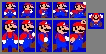
\includegraphics[width=5cm]{figuras/SpritesMario.png}
	\caption{Sprites Mario}
	\label{image: Sprites Mario}
\end{figure}

Entre as imagens que representam o movimento, o caso da corrida é diferente do pulo por ter três imagens para representar seu movimento. Durante a movimentação do personagem essas três imagens são mostradas em sequência para transmitir a sensação de movimento, tal como o jogo original faz. 

Para a implementação da música, os códigos de referência previamente citados foram aplicados. A grande diferença providenciada por esses códigos está ligada a possibilidade da execução da música sem paralisar a execução das demais partes do código, o que é feito reunindo as notas a serem tocadas em um vetor que será percorrido um elemento por execução do loop principal do jogo.

Utilizando da mesma ideia os efeitos sonoros foram aplicados. O principal efeito sonoro colocado no jogo foi o som indicativo de morte. Ao jogador cair em um buraco que leva ao fim do mapa, o sprite é trocado para o sprite de morte e uma música específica é tocada antes da finalização do programa.

\subsection{Arte}
\label{Artes}
\indent \indent A parte da arte do jogo abrange muito mais do que apenas as animações do personagem, dos inimigos e do Power-Up apresentado. Para a confecção do mapa em forma matricial, foi necessário a divisão de diversas imagens diferentes que pudessem representar cada bloco do mapa.

Os principais blocos utilizados podem ser vistos na imagem \ref{image: Blocos do mapa}.

\begin{figure}[H]
	\centering
	
\includegraphics[width=3cm]{figuras/Blocos.png}
	\caption{Blocos do mapa}
	\label{image: Blocos do mapa}
\end{figure}

Para confecção da arte do personagem e inimigos, foram utilizadas, como referência, as artes do próprio jogo original, encontradas nas seções de “Playable Characters” e “Enemies \& Bosses” da referência \cite{Sprites}. 

\begin{figure}[H]
	\centering
	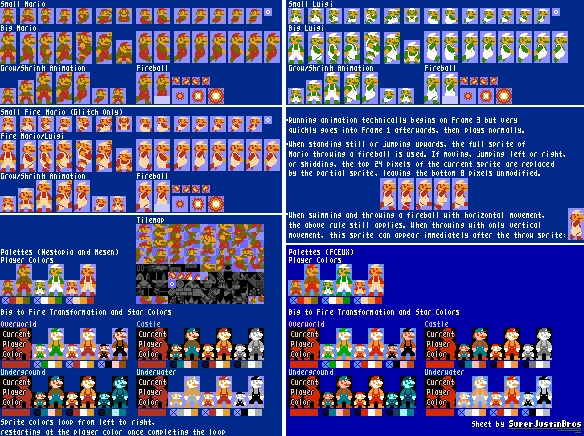
\includegraphics[width=6cm]{figuras/Personagens1.jpeg}
	\caption{Tabela de Personagens}
	\label{image: Tabela de Personagens1}
\end{figure}

\begin{figure}[H]
	\centering
	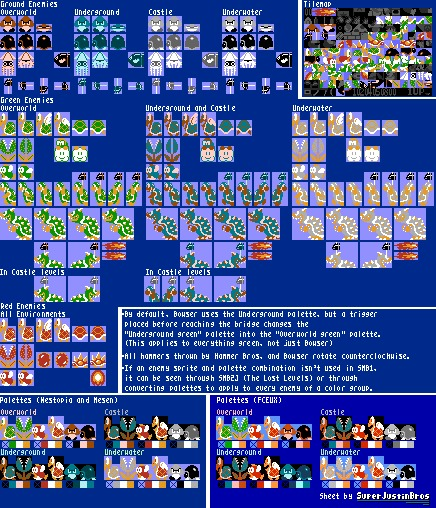
\includegraphics[width=5cm]{figuras/Personagens2.jpeg}
	\caption{Tabela de Personagens}
	\label{image: Tabela de Personagens2}
\end{figure}

Apesar dos inimigos seguirem fielmente as artes originais, o personagem Mario segue outra abordagem. Neste trabalho, o Mario preserva suas dimensões e formato da obra original, entretanto, sua paleta de cores foi alterada para seu visual mais “familiar”. Tal visual foi inspirado pelas suas artes no jogo Super Mario World (Nintendo, 1990) e no filme Super Mario Bros. O Filme (Universal Pictures; Nintendo; Illumination Entertainment, 2023).

\begin{figure}[H]
	\centering
	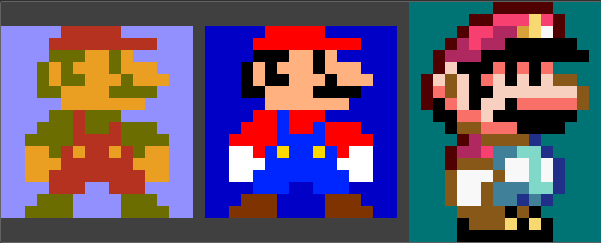
\includegraphics[width=5cm]{figuras/comparacao_sprites.png}
	\caption{Comparação dos Sprites}
	\label{image: Comparacao dos Sprites}
\end{figure}

Assim como os inimigos, as telas do trabalho seguem inspiração direta das telas do jogo original, como as telas de “game over” e vitória. Elas foram criadas a partir da referência \cite{Sprites} nas seções de “Backgrounds”, para os detalhes do menu principal, e “Miscellaneous”, onde a disponibilidade das fontes de texto nesta seção foram essenciais para a criação de telas dependentes de texto, como a tela de enredo. A tela de enredo apresenta uma breve contextualização ao jogador de qual é o seu objetivo: salvar a Princesa Peach do Bowser; objetivo no qual é recorrente na maioria dos jogos da franquia Mario.

\begin{figure}[H]
	\centering
	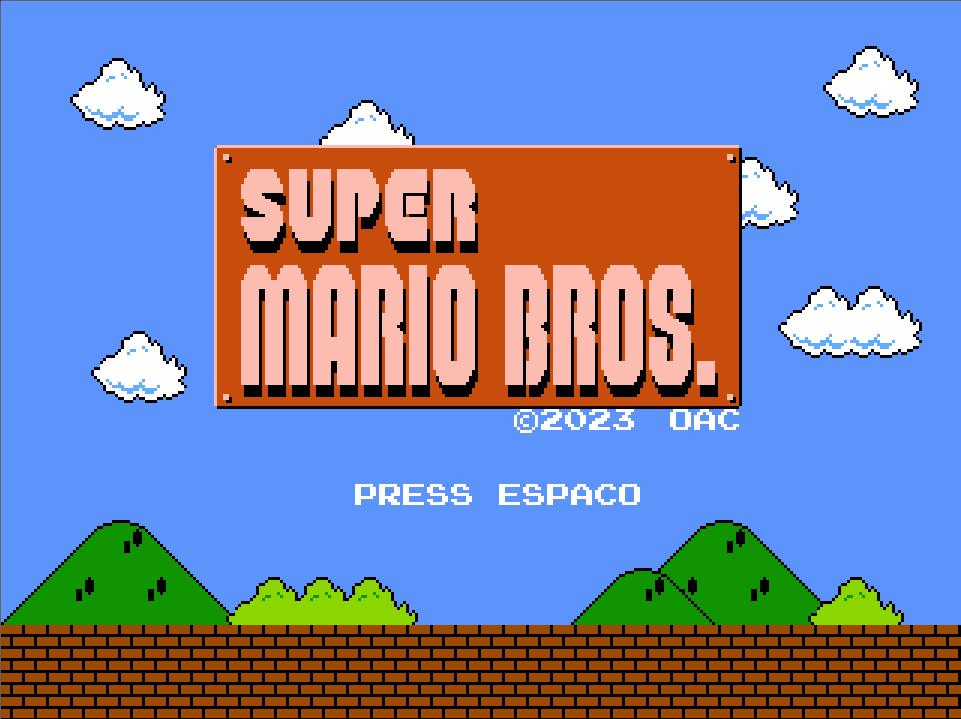
\includegraphics[width=5cm]{figuras/menu_principal.png}
	\caption{Tela Principal}
	\label{image: Tela Principal}
\end{figure}

\begin{figure}[H]
	\centering
	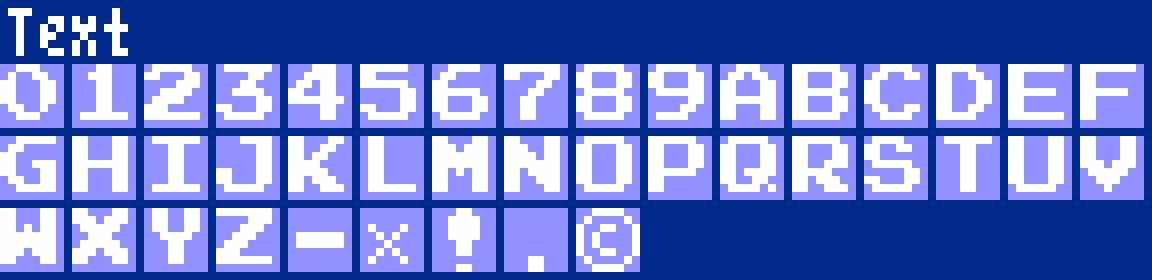
\includegraphics[width=5cm]{figuras/fonte_de_texto.png}
	\caption{Fontes de texto}
	\label{image: Fontes de texto}
\end{figure}

\begin{figure}[H]
	\centering
	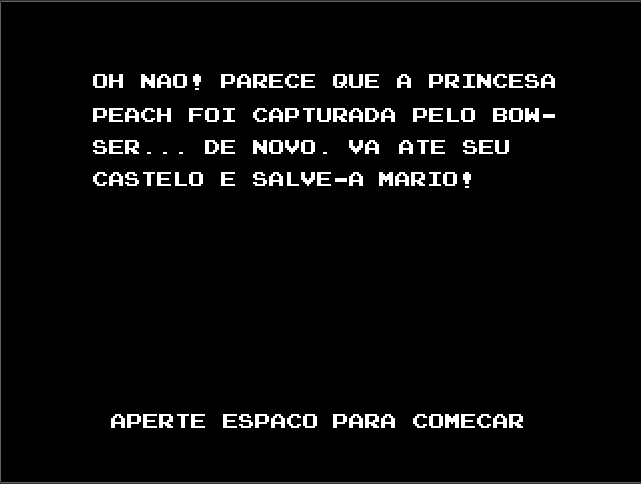
\includegraphics[width=5cm]{figuras/tela_enredo.png}
	\caption{Tela de Enredo}
	\label{image: Tela de Enredo}
\end{figure}


\section{Resultados Obtidos}
\indent \indent Após toda a confecção e testes, existem diversos resultados que são importantes de citar ao serem obtidos com a confecção desse jogo. O primeiro resultado obtido foi a impossibilidade da implementação de tudo que foi planejado em tempo hábil. Diversas funcionalidades que foram analisadas do jogo original não puderam ser implementadas devido a imprevistos ao longo do desenvolvimento. 

Entre as funcionalidades que foram analisadas e não puderam ser implementadas está a vida extra que seria dada pelo cogumelo, que só foi capaz de trocar a aparência do personagem. Outra mecânica que não foi implementada é o final do nível, pois a fase apenas buscou demonstrar todas as mecânicas implementadas, o que levou a inexistência de uma região que fosse determinada como um final para a obtenção da tela de vitória.

Além das mecânicas que não puderam ser implementadas, também existiram aprendizados importantes que puderam ser considerados no desenvolvimento do jogo. Ao estar usando uma linguagem de baixo nível, é de extrema importância os comentários documentando tudo que está sendo feito, além do cuidado com os usos dos registradores, os quais podem ser facilmente sobrescritos, levando a erros catastróficos na execução do programa.

Quanto ao uso de memória, foi observado durante o desenvolvimento que buscar minimizar os gastos implica em um ganho equivalente de complexidade. Este fato pode ser observado na utilização de uma matriz de blocos para a construção do mapa do jogo. Ao utilizar tal recurso, todo o sistema de movimentação, colisão e inimigos precisou ser adaptado para que o movimento dos personagens se mantivesse suave (movimentos de 2 pixeis por frame) ao contrário dos movimentos bruscos que a matriz inicialmente impunha (movimentos de 16 pixeis).

Dessa forma, o trabalho cumpriu com seus objetivos de analisar a aplicação do Assembly RISC-V para o desenvolvimento de um jogo em conjunto com o gasto reduzido de memória. 

\section{Conclusões}
\indent \indent Desse modo, podemos concluir que as mecânicas principais do jogo são simples de identificar, no entanto a implementação requer uma quantidade considerável de tempo e um esforço maior do que as ideias transmitem.

Dessa forma, a utilização de uma linguagem de baixo nível possibilita um ganho considerável de eficiência, se usada de maneira adequada, mas na mesma medida é capaz de dificultar o desenvolvimento. 

Outro ponto importante que pode ser considerado é a dificuldade associada as limitações de memória impostas para o desenvolvimento deste trabalho. Ao impor um espaço extremamente limitado, são levantados diversas dinâmicas de otimização, reaproveitamento e relacionados que são de grande importância no desenvolvimento de projetos. 

Nesse sentido, o desenvolvimento desse trabalho conseguiu servir com seu propósito de estudar as dinâmicas envolvidas no desenvolvimento em linguagens de baixo nível e com limitações perceptíveis de memória.

\begin{thebibliography}{3}
	\bibitem[1]{Sprites}{NES - Super Mario Bros. The Spriters Resource. Acesso em: 17 de jul. de 2023. Disponível em: https://www.spriters-resource.com/nes/supermariobros/}
	\bibitem[2]{Pulsar}{Araujo, V. Vini-ara/pulsar-sega: Pulsar sega game wirtten in RISC-V assembly. GitHub. Acesso em: 17 de jul. de 2023. Disponível em: https://github.com/Vini-ara/Pulsar-Sega}
	\bibitem[3]{Hooktheory}{Patury, D. (2020). Hooktheory to RISC-V midi. Gist. Acesso em: 17 de jul. de 2023. Disponível em: https://gist.github.com/davipatury/ cc32ee5b5929cb6d1b682d21cd89ae83}
\end{thebibliography}
		
\end{document}
